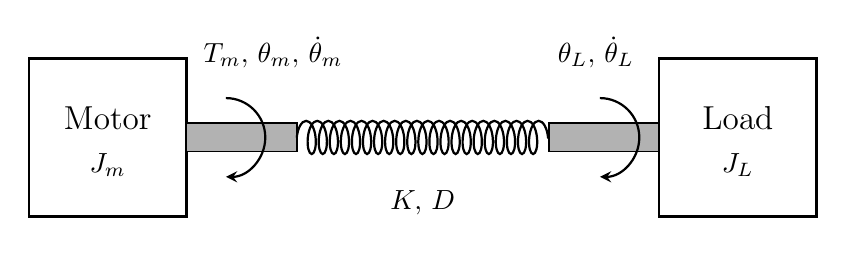
\begin{tikzpicture}[>=stealth, thick]

  % Motor box
  \draw[line width=1pt] (-5,  -1.0) rectangle (-3,  1.0);
  \node at (-4, 0.25) {\large Motor};
  \node at (-4,-0.35) {$J_m$};

  % Motor shaft (left segment)
  \draw[fill=gray!60, draw=black, line width=0.6pt]
    (-3, 0.18) rectangle (-1.6, -0.18);

  % Spring (coil) in the middle
  \draw[decoration={coil, aspect=0.4, segment length=4pt, amplitude=6pt},
        decorate, line width=0.8pt]
    (-1.6, 0) -- (1.6, 0);

  % Load shaft (right segment)
  \draw[fill=gray!60, draw=black, line width=0.6pt]
    (1.6, 0.18) rectangle (3, -0.18);

  % Load box
  \draw[line width=1pt] (3, -1.0) rectangle (5, 1.0);
  \node at (4, 0.25) {\large Load};
  \node at (4,-0.35) {$J_L$};

  % Motor-side labels: T_m, theta_m, omega_m
  \node[above] at (-1.9, 0.75) {$T_m,\,\theta_m,\,\dot{\theta}_m$};

  % Motor-side rotation arrow: half-circle from noon, arrowhead pointing down
  \draw[->, line width=0.8pt]
    (-2.5, 0.5) arc[start angle=90, end angle=-90, radius=0.5];

  % Load-side labels: theta_L, omega_L
  \node[above] at (2.2, 0.75) {$\theta_L,\,\dot{\theta}_L$};

  % Load-side rotation arrow: half-circle from noon, arrowhead pointing down
  \draw[->, line width=0.8pt]
    (2.25, 0.5) arc[start angle=90, end angle=-90, radius=0.5];

  % Spring label K, D
  \node[below] at (0, -0.55) {$K,\,D$};

\end{tikzpicture}
